% !TeX root = ../note.tex
\section{Разработка программного средства}\label{sec:development}

Разработанное программное обеспечение представляет из себя набор сервисов, необходимых для развёртывания криптовалютной биржи, написанное на языке Golang.

\subsection{Общая схема взаимодействия сервисов}

\begin{figure}[ht]
    \centering
    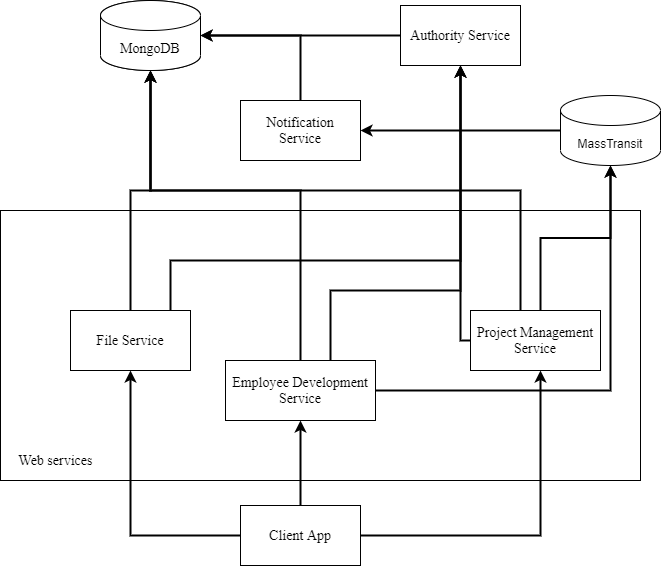
\includegraphics[width=\textwidth]{general_scheme}
    \caption{Схема взаимодействия сервисов}\label{fig:general_scheme}
\end{figure}

На рисунке~\ref{fig:general_scheme} изображена схема взаимодействия сервисов программного средства.

Для взаимодействия с системой пользователю необходимо зарегистрироваться и авторизоваться. Для этих целей используется Authority service. Регистрация и изменение аккаунтов происходят посредством RabbitMQ, чтобы гарантировать доставку сообщений. Аутентификация пользователей происходит через RPC запросы. Также данный сервис возвращает события об изменении аккаунтов. Все запросы, вызывающие изменение баланса, передаются посредством RabbitMQ. Это необходимо для того, чтобы не потерять сообщения и в случае отказа сервиса восстановить состояние slave-сервера.

Получение информации о балансах происходит посредством RPC запроса. Из-за высокой нагрузки на этот модуль одному типу валюты должен соответствовать один сервис. Также balances service может шардироваться. Данный сервис возвращает события об изменении балансов. Для создания, удаления и матчинга ордеров используется Matching service. Один сервис соответствует одной паре валют. Информация о создаваемом ордере передается через RabbitMQ. При закрытии ордера сервис отправляет сообщение об изменении балансов на Balances Services через RabbitMQ и выкидывает событие на Node. Каждый сервис является самодостаточным и сам разрешает внутренние отказы.

Для добавления любого нового сервиса (Matching service, Balances service) необходимо поднять сам сервис, зарегистрировать его в Nodes. Balances service и Authority service могут поддерживать sharding. Добавляется точно такой же сервис, а распределение между шардами будет происходить на уровне выше (Node или proxy).

\subsection{Сервис матчинг}\label{sec:development:matching}

Данный сервис занимается сопоставлением ордеров, сохранением результатов в базы данных и извещением клиентов об операциях над ордерами.

\begin{figure}[ht]
    \centering
    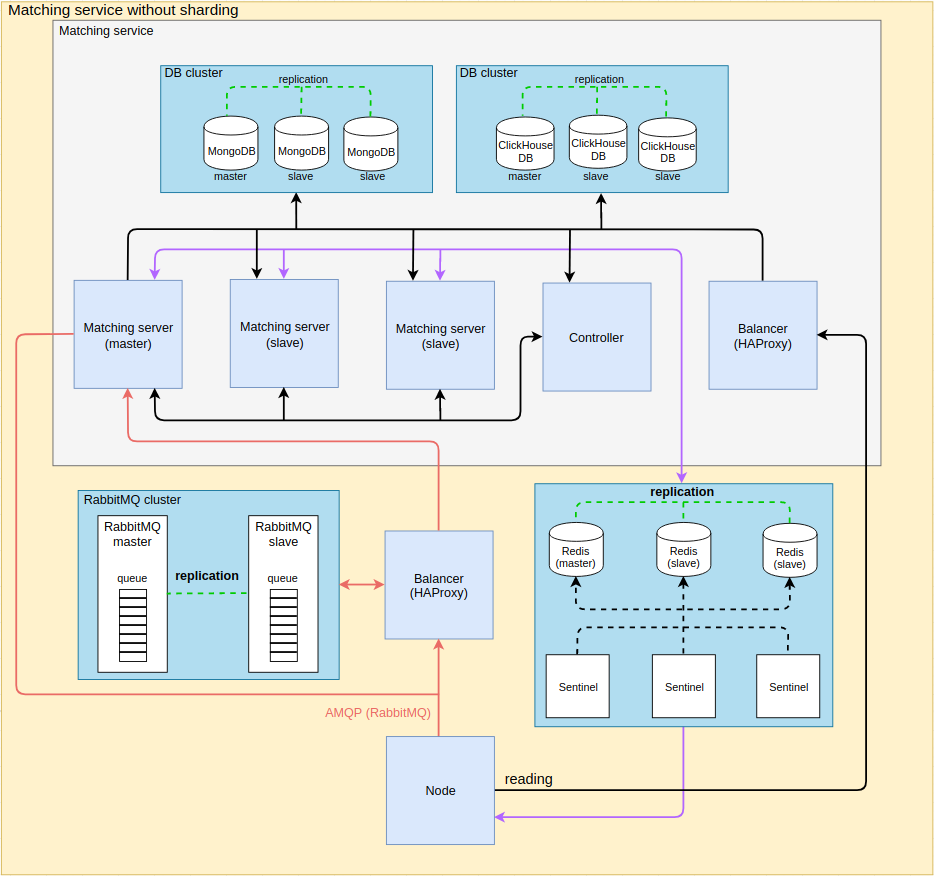
\includegraphics[width=\textwidth]{matching_service}
    \caption{Схема работы сервиса матчинга}\label{fig:matching_service}
\end{figure}

Сервис хранит необходимую информацию, необходимую для обработки ордера, в оперативной памяти с целью обеспечения более быстрого доступа.
Информация об ордерах и проведённых сделках хранится в соответствующих базах данных.
Все главные модули работают в разных потоках.
Также для обеспечения быстрой работы используются буферизация и пакетная запись в базу.

% \subsubsection{} Алгоритм обработки ордеров
\textbf{Алгоритм обработки ордеров}

Создание, удаление ордеров происходят следующим образом:
\begin{enumerate}
    \item Node отправляет сообщение на Matching Server посредством RabbitMQ. Подключение к RabbitMQ происходит через HAProxy, это необходимо, так как мы используем кластер из RabbitMQ серверов. HAProxy отвечает за установление tcp-соединения с текущим master RabbitMQ и перенаправление нового tcp-соединения на новый master, если старый master RabbitMQ перестал работать. RabbitMQ содержит только одну очередь.
    \item Сообщение кладётся в текущий master RabbitMQ, с которой Node установило tcp-соединение.
    \item Matching master-сервер подключается тем же способом, что и Node, для чтения сообщений и обработки их.
    \item Matching master-сервер отправляет данные через mongodb-diver на запись в кластер MongoDB.
    \item После того как данные записались в master, происходит репликация баз.
    \item Кластер MongoDB настроен таким образом, что подтверждение о записи в базу данных будет приходить после записи данных на все сервера кластера.
    \item После записи данных в базу master-сервер отправляет событие об успешном выполнении операции и отправляет подтверждение на RabbitMQ о том, что сообщение было обработано и может быть удалено из очереди. Отправляется запрос на изменение балансов в необходимые Balances services.
    \item Slave-сервера слушают события от master-сервера, и после получения события, дублируют информацию в оперативной памяти.
    \item Node так же слушает события отправленные master-сервером. Чтение происходит следующим образом: Node обращается непосредственно к кластеру баз данных. Отправляет запрос на подключение через HAProxy балансер, который распределяет все поступившие запросы на все базы в кластере, тем самым распределяя нагрузку на все базы в кластере.
\end{enumerate}

% \subsubsection{} Падение Matching master-сервера
\textbf{Падение Matching master-сервера}

Сontroller проверяет с заданным интервалом доступность всех Matching server. Если Сontroller не получит ответ от master-сервера в заданный промежуток времени — это будет означать, что сервер недоступен. В этом случае Сontroller должен переключить один из slave-серверов в master. Controller выбирает один из slave-серверов и посылает ему gRPC запрос о том, что ему необходимо переключиться в master режим.

% \subsubsection{} Описание модулей
\textbf{Описание модулей}

В состав сервиса входит 5 основных модулей:

% \begin{enumerate}
    % \item Обработка входящих сообщений (\ref{sec:development:net});
    % \item Сопоставление ордеров или матчинг (\ref{sec:development:match});
    % \item База ордеров (\ref{sec:development:order});
    % \item База сделок (\ref{sec:development:trade});
    % \item Обновление балансов (\ref{sec:development:balance});
    % \item События (\ref{sec:development:events});
    % \item Восстановление данные (\ref{sec:development:restore}).
% \end{enumerate}

\begin{enumerate}
    \item Обработка входящих сообщений;
    \item Сопоставление ордеров или матчинг;
    \item База ордеров;
    \item База сделок;
    \item Обновление балансов;
    \item События;
    \item Восстановление данные.
\end{enumerate}

Также используются несколько дополнительных модулей:

% \begin{enumerate}
%     \item Логирование (\ref{sec:development:logs});
%     \item Интерфейс командной строки (\ref{sec:development:cli});
%     \item Конфигурация (\ref{sec:development:config}).
% \end{enumerate}

\begin{enumerate}
    \item Логирование;
    \item Интерфейс командной строки;
    \item Конфигурация.
\end{enumerate}

% \subsubsection{} Обработка входящих сообщений\label{sec:development:net}
\textbf{Обработка входящих сообщений}

В качестве интерфейса для получения сообщений используется RabbitMQ.
Входящие сообщения считываются из очереди в RabbitMQ, десериализуются и помещаются в очередь на обработку.
Для сериализации используется protobuf.

% \subsubsection{} Сопоставление ордеров (матчинг)\label{sec:development:match}
\textbf{Сопоставление ордеров (матчинг)}

Схема получения ордеров и отправления результатов изображена на рисунке~\ref{fig:matching_engine}

\begin{figure}[ht]
    \centering
    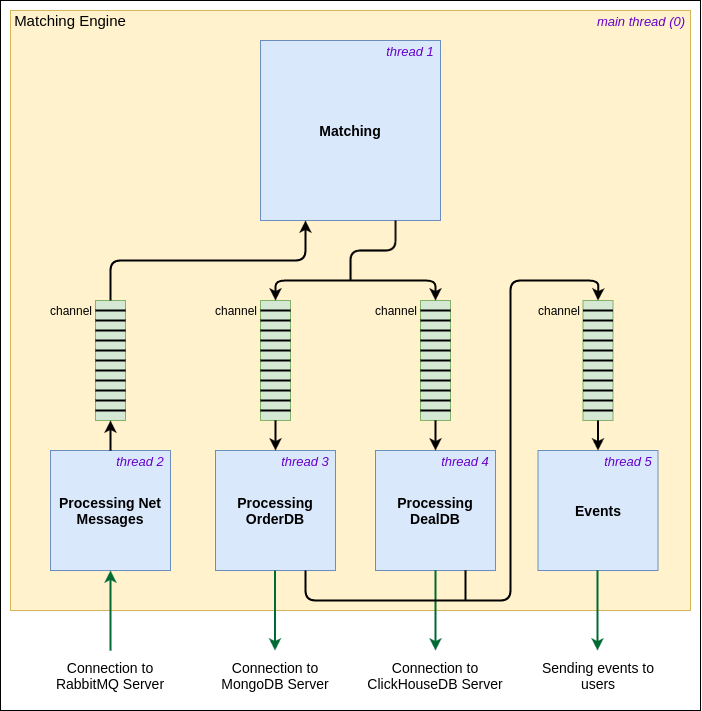
\includegraphics[width=\textwidth]{matching_engine}
    \caption{Обработка ордеров}\label{fig:matching_engine}
\end{figure}

Новый ордер считывается из очереди на обработку. Сопоставление проходит в два этапа:

\begin{enumerate}
    \item Поиск подходящих ордеров
    \item Обновление информации об ордерах в оперативной памяти
\end{enumerate}

Для хранения и поиска используется контейнер ордеров, который приведён на листинге~\ref{list:container}, содержащий три структуры данных:

\begin{enumerate}
    \item Словарь с ордерами, и их идентификаторов в качестве ключей — нужен для обеспечения быстрого доступа к ордерам
    \item Словарь, в котором в качестве ключей используются цены ордеров, а значения — массивы идентификаторов ордеров с данной ценой.
    \item Отсортированное множество цен всех ордеров
\end{enumerate}

\lstinputlisting[caption=Состав контейнера и его инициализация,language=Golang,label={list:container}]{appendix/container.go}

Интерфейс контейнера ордеров:

\begin{itemize}
    \item \lstinline{Add(order *models.Order)} — добавление ордера в контейнер. Ордер будет добавлен по очереди во все три внутренних контейнера;
    \item \lstinline{Empty() : bool} — проверка на наличие хотя бы одного ордера в контейнере. Проверка проходит по всем трём контейнерам, и если все будут пустыми, то вернётся положительный результат;
    \item \lstinline{FindMatches(order *models.Order) : []int64} — поиск ордеров в контейнере, которые могут создать сделку с данным ордером. Если существует несколько ордеров способных закрыть полученный ордер, то все они учитываются. Итогом работы функции является массив из идентификаторов всех ордеров, с которыми смог совершить сделки данный ордер.
    \item \lstinline{GetOrderByID(id int64) : models.Order, bool} — ищет ордер в контейнере по данному идентификатору. Возвращает два значения: найденный ордер или пустой ордер, если ничего не нашло, а второе значение — булевое значение, показывающее нашло ли ордер по данному идентификатору;
    \item \lstinline{Initialize(comparator utils.Comparator)} — инициализирует внутренние контейнеры с данным компаратором. Описание работы компараторов приведено ниже;
    \item \lstinline{ModifyOrderValue(id int64, value uint64) : models.Order, bool} — используется для обновления значения объема средств ордера, доступных для продажи или покупки;
    \item \lstinline{Remove(id int64) : error} — удаление ордера из контейнеров. Метод может вернуть ошибку, если данного ордера нет в контейнере.
\end{itemize}

Компараторы необходимы для функционирования контейнеров на продажу и покупку, так как они действуют по схожему алгоритму, но обязаны сортировать ордеры внутри себя в обратных друг другу последовательностях. Пример компаратора приведен в листинге~\ref{list:comparator}. Компаратор принимает на вход два значения, которые должны конвертироваться в целые положительные числа.

\lstinputlisting[caption=Примеры компараторов,language=Golang,label={list:comparator}]{appendix/comparator.go}

Алгоритм обработки нового ордера:

\begin{itemize}
    \item Перед началом обработки ордеров создаются два контейнера ордеров, в одном хранятся ордеры для продажи, в другом — для покупки.
    \item При поступлении ордера на покупку, поиск подходящих ордеров происходит в контейнере с ордерами на продажу и наоборот.
\end{itemize}

\begin{enumerate}
    \item Ищем все ордера, суммарной стоимости которых хватит на то, чтобы максимально закрыть новый ордер.
Таких ордеров может быть как много, так и ни одного.
В случае, если для нового ордера не было найдено ордеров для совершения сделки, он добавляется в контейнер ордеров, и ждёт, пока не появится подходящий ордер.

    \item Непосредственно поиск производится с помощью множества цен ордеров.
Если новый ордер выставлен на покупку, то из отсортированного множества цен берется самая маленькая цена в контейнере ордеров на продажу (и наоборот в случае, если новый ордер — на продажу).
Если самая маленькая (большая) цена больше (меньше) цены ордера, то сделок произведено не будет, потому что для нового ордера такая сделка будет убыточной, а ордер впоследствии будет добавлен в контейнер, чтобы ожидать новых ордеров.

    \item Если с минимальной (максимальной) ценой всё в порядке, то выбираются ордеры с данной ценой (с помощью словаря цен/массив идентификаторов) и проверяется, хватит ли суммы выбранных ордеров для закрытия нового ордера.
Если не хватило ордеров, чтобы полностью закрыть новый ордер, то смотрим на ордеры с ценой выше (ниже), пока эта цена меньше (больше) цены ордера.
Когда средств становится достаточно или когда ордера для сделки заканчиваются, отправляем полученный массив ордеров для создания сделок.

    \item Присваиваем новому ордеру идентификатор.
Производим сделки между новым ордером и подходящими ему ордерами.
Если новый ордер не закрылся, то добавляем его в соответствующий контейнер.
Все ордера, которые закрылись в результате сделок, удаляем из контейнера (тем самым очищаем память).
\end{enumerate}

В результате алгоритма получаем новый ордер, который может быть частично или полностью закрыт, массив обновленных ордеров и массив сделок. Всё эти данные отправляются дальше для записи в базу данных.

% \subsubsection{} База ордеров\label{sec:development:order}
\textbf{База ордеров}

Модель ордера для базы данных и для работы внутри сервиса приведены в листинге~\ref{list:orders}.

\lstinputlisting[caption=Модели ордеров для базы данных и внутреннего использования,language=Golang,label={list:orders}]{appendix/order.go}

В качестве базы для хранения ордеров используется mongoDB. Для сохранения данных используются псевдонимы для полей структуры, которые написаны в кавычках после объявлений полей с тегом \lstinline{bson}. BSON (от Binary JavaScript Object Notation) — бинарная форма представления простых структур данных и ассоциативных массивов. Является надмножеством JSON, включая дополнительно регулярные выражения, двоичные данные и даты.

Для сохранения данных в базе используется пакетная запись.
После матчинга в базу нужно записать новый ордер и обновить ордеры, с которыми совершены сделки.
Новый ордер кладётся в буфер для записи в базу, а обновлённые ордеры — в буфер для обновления базы.
Данные буферы отправляют содержимое в базу для обработки при двух условиях:

\begin{itemize}
    \item по достижении таймаута на запись в буфер (то есть через определённые промежутки времени буфер очищается)
    \item при заполнении буфера
\end{itemize}

Возможна ситуация, когда один и тот же ордер может оказаться и в буфере для записи, и в буфере для обновлении.
Поэтому при добавлении ордера в буфер для обновления, проверяется, есть ли он в очереди на запись.
Если нету, то он просто добавляется в буфер.
Иначе он добавляется в очередь на обновление, которая переместит своё содержимое в буфер после очередного таймаута.

% \subsubsection{} База сделок\label{sec:development:trade}
\textbf{База сделок}

В качестве базы для хранения сделок используется ClickhouseDB.

Для сохранения данных в базу сделок также используется пакетная запись.
После матчинга в базу записываются все проведённые сделки.
Сделке присваивается идентификатор перед отправлением в буфер на запись.
Буфер очищается так же, как и буферы для базы ордеров:

\begin{itemize}
    \item по таймауту;
    \item при заполнении буфера.
\end{itemize}

% \subsubsection{} Обновление балансов\label{sec:development:balance}
\textbf{Обновление балансов}

При совершении сделки в сервис балансов отправляются четыре сообщения об обновлении балансов пользователей. Два сообщения указывают, сколько и каких средств у пользователей нужно снять, ещё два указывают, сколько нужно добавить. Сообщения посылаются в двух очередях через RabbitMQ.

% \subsubsection{} События\label{sec:development:events}
\textbf{События}

События отправляются через Redis (используется в качестве ``шины''). Отправка идёт по каналам, доступные каналы:

\begin{itemize}
    \item CreatedOrder — ордер создан;
    \item UpdatedOrder — ордер обновлён;
    \item RemovedOrder — ордер удалён;
    \item CreatedTrade — произошла сделка;
    \item Error — произошла ошибка;
\end{itemize}

Данные в событии представляют собой сериализованный в JSON объект (ордер или сделка).
По каналу Error приходит JSON массив, первый элемент в котором string с ошибкой, второй — объект, вызвавший ее.
События сериализуются с помощью protobuf. Каждое событие имеет уникальный идентификатор.
Сервер сообщений работает в отдельном потоке.
По всем каналам, кроме ``Updated'' приходят события в виде JSON массива (внутри лежат объекты JSON).

% \subsubsection{} Восстановление данные\label{sec:development:restore}
\textbf{Восстановление данные}

Максимально быстрая работа базы данных достигается за счёт хранения данных в оперативной памяти во время исполнения. При аварийном запуске или запланированной остановке сервисов, необходимо не потерять данные после перезапуска, потому что все сделки — это реальные финансы клиентов. Для достижения этой цели клиент для базы данных реализовывает интерфейс восстановления ордеров. Суть сводится к тому, чтобы для контейнера покупки или продажи достать все незакрытые ордера и сконвертировать их в ордера для внутреннего хранения. Реализация восстановления ордеров из базы данных приведена на листинге~\ref{list:restore-orders}.

\lstinputlisting[caption=Восстановление ордеров,language=Golang,label=list:restore-orders]{appendix/restore.go}

% \subsubsection{} Логирование\label{sec:development:logs}
\textbf{Логирование}

Logger имеет интерфейс, предоставляющий API логирования различного уровня.
Доступные уровни:

\begin{itemize}
    \item debug — информация для отладки программы;
    \item info — уровень ``общей'' информации;
    \item warn — предупреждение об неправильном поведении;
    \item error — ошибка, позволяющая продолжить работу;
    \item crit — критическая ошибка, завершающая работу программы.
\end{itemize}

Уровни идут по возрастанию значимости (следовательно, если выставлен уровень info, то логи уровня debug выводиться не будут).

Logger записывает логи уровня error и crit в файл, переданный через конфиг. Эти данные записываются в JSON формате. Так же Logger выводит в stdout логи заданного, через конфиг, уровня, данные логи идут в fmt формате. Каждая запись в логах имеет сообщения вида \lstinline{caller=<caller_file>} — файл и строка, вызвавшие лог и \lstinline{func=<caller_func>} — название функции, вызвавшей лог.

Благодаря реализации на интерфейсе, Logger имеет возможно быстро подменять своё ядро реализации. В данный момент используется библиотека log15.

% \subsubsection{} Интерфейс командной строки\label{sec:development:cli}
\textbf{Интерфейс командной строки}

Исполняемый файл предоставляет возможность передачи аргументов через командную строку. Можно провести полную конфигурацию через командную строку. Возможные аргументы можно просмотреть используя \lstinline{--help} (полноценное сообщение приведено на листинге~\ref{list:help-matching}). Каждый аргумент имеет значения по умолчанию, так же аргументы командной строки имеют более высокий приоритет, чем конфигурационный файл (если задан один и тот же параметр в конфигурационном файле и в командной строке, будет использовано значение параметра из командной строки).

\lstinputlisting[caption=Справка для help флага,label=list:help-matching]{appendix/help.txt}

% \subsubsection{} Конфигурация\label{sec:development:config}
\textbf{Конфигурация}

Так же предоставляется возможность конфигурации через файл \lstinline{*.yml}. Его работа устроена так же как и с аргументами командной строки, отличие только в том, что аргументы командной строки имеют более высокий приоритет

Пример подобного конфиг файла на листинге~\ref{matching-config}.

\lstinputlisting[caption=Пример YAML конфига матчинг сервиса,label=matching-config]{appendix/matching-config.yml}

\subsection{Сервис балансов}

В сервис балансов также входят различные модули, некоторые из которых были описаны в разделе~\ref{sec:development:matching}.

% \begin{enumerate}
%     \item Обработка входящих сообщений (\ref{sec:development:net});
%     \item База балансов (\ref{sec:development:db_balance});
%     \item События (\ref{sec:development:events});
%     \item Восстановление данные (\ref{sec:development:restore}).
% \end{enumerate}

\begin{enumerate}
    \item Обработка входящих сообщений;
    \item База балансов;
    \item События;
    \item Восстановление данные.
\end{enumerate}

Также используются несколько дополнительных модулей, описанных ранее:

% \begin{enumerate}
%     \item Логирование (\ref{sec:development:logs});
%     \item Интерфейс командной строки (\ref{sec:development:cli});
%     \item Конфигурация (\ref{sec:development:config}).
% \end{enumerate}

\begin{enumerate}
    \item Логирование;
    \item Интерфейс командной строки;
    \item Конфигурация.
\end{enumerate}

% \subsubsection{} База балансов\label{sec:development:db_balance}
\textbf{База балансов}

Для записи данных в базу балансов используется такой же клиент для MongoDB, который использовался в сервисе матчинга. Для быстроты работы данные также, как и в матчинг сервисе хранятся в оперативной памяти. На листинге~\ref{list:cache} приведена структура кеша.

\lstinputlisting[caption=Структура кеша балансов,language=Golang,label=list:cache]{appendix/cache.go}

\begin{figure}[ht]
    \centering
    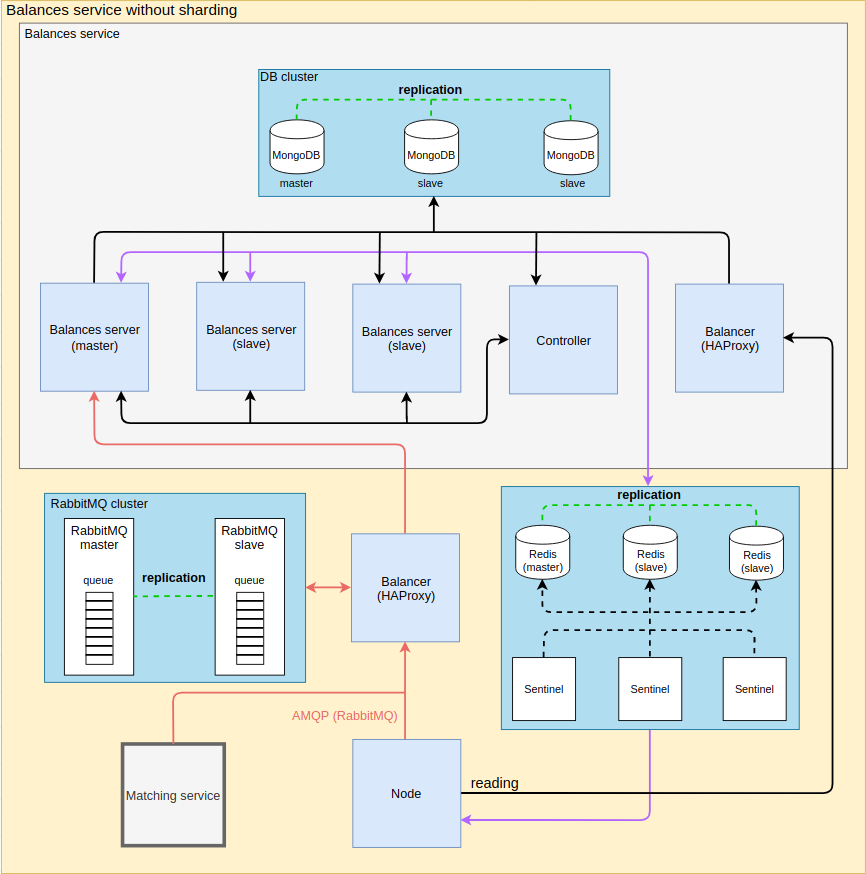
\includegraphics[width=\textwidth]{balances_service}
    \caption{Схема работы сервиса балансов}\label{fig:balances_service}
\end{figure}

% \subsubsection{} Обработка изменения балансов
\textbf{Обработка изменения балансов}

Пополнение, вывод, заморозка, разморозка, перевод балансов происходят следующим образом:
\begin{enumerate}
    \item Node или Matching service отправляет сообщение на Balances Server посредством RabbitMQ. Подключение к RabbitMQ происходит через HAProxy. Это необходимо, так как мы используем кластер из RabbitMQ серверов. HAProxy отвечает за установление tcp-соединения с текущим master RabbitMQ и перенаправление нового tcp-соединения на новый master, если старый master RabbitMQ перестал работать. RabbitMQ содержит только одну очередь.
    \item Сообщение кладётся в текущий master RabbitMQ, с которой Node установило tcp-соединение.
    \item Balances master-сервер подключается тем же способом, что и Node, для чтения сообщений и обработки их.
    \item Balances master-сервер отправляет данные через mongodb-driver на запись в кластер MongoDB.
    \item После того как данные записались в master, происходит репликация баз.
    \item Кластер MongoDB настроен таким образом, что подтверждение о записи в базу данных будет приходить после записи данных на все сервера кластера.
    \item После записи данных в базу master-сервер отправляет событие об успешном выполнении операции и отправляет подтверждение на RabbitMQ о том, что сообщение было обработано и может быть удалено из очереди.
    \item Slave-сервера слушают события от master-сервера, и после получения события, дублируют информацию в оперативной памяти.
    \item Node также слушает события, отправленные master-сервером. Чтение происходит следующим образом: Node обращается непосредственно к кластеру баз данных. Отправляет запрос на подключение через HAProxy балансер, который распределяет все поступившие запросы на все базы в кластере, тем самым распределяя нагрузку на все базы в кластере. Каналы сообщений в Redis: ``DepositBalance'', ``WithdrawalBalance'', ``FreezingBalance'' и ``UnfreezingBalance''.
\end{enumerate}

% \subsubsection{} Падение Balances master-сервера
\textbf{Падение Balances master-сервера}

Controller проверяет с заданным интервалом доступность всех Balances server. Если Controller не получит ответ от master-сервера в заданный промежуток времени — это будет означать, что сервер недоступен. В этом случае Controller должен переключить один из slave-серверов в master. Controller выбирает один из slave-серверов и посылает ему RPC запрос о том, что ему необходимо переключиться в master режим.

\subsection{Сервис аутентификации}

\begin{figure}[ht]
    \centering
    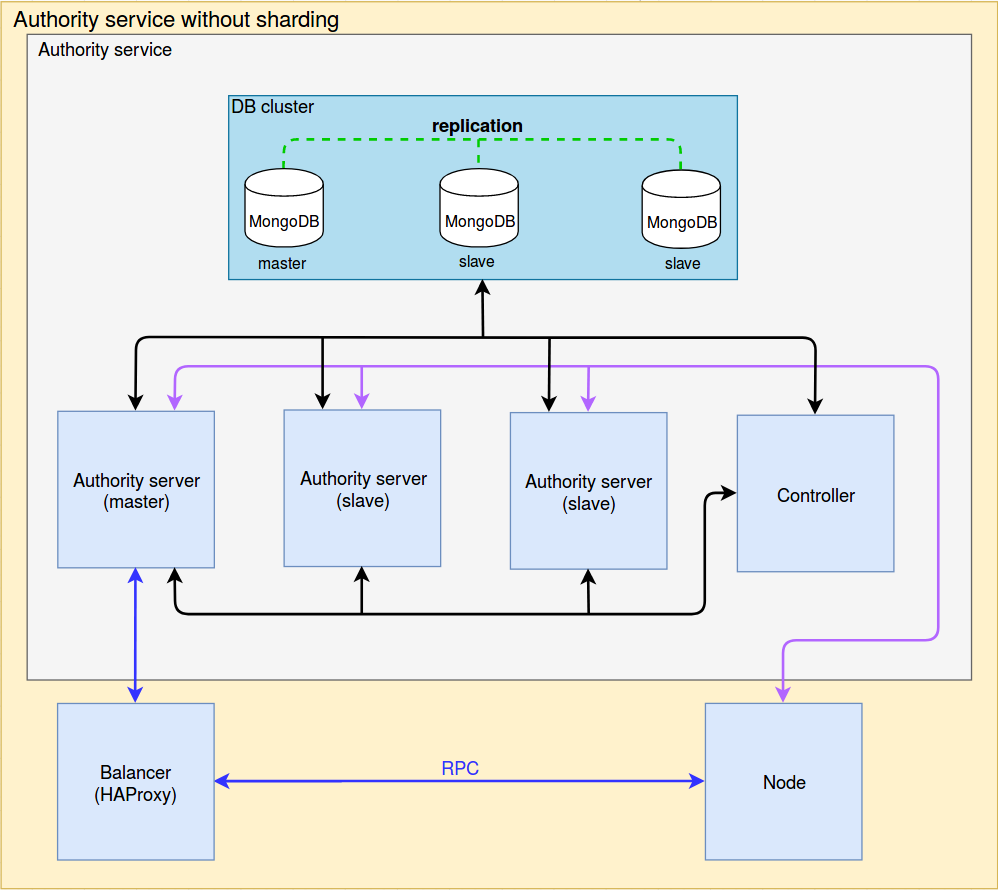
\includegraphics[width=\textwidth]{authority_service}
    \caption{Схема работы сервиса аутентификации}\label{fig:authority_service}
\end{figure}

% \subsubsection{} Интерфейс для взаимодействия сервисом
\textbf{Интерфейс для взаимодействия сервисом}

\begin{itemize}
    \item \lstinline{AuthUser(login string, password string) : models.AccountModel, error} — аутентификация пользователя по логину и паролю;
    \item \lstinline{DeleteUser(userid int64) : error} — удаление пользователя из базы. При отсутствии пользователя возвращается ошибка;
    \item \lstinline{GetAuthServerPubkey() : string} — получение публичного ключа x509;
    \item \lstinline{GetUserByID(userID int64) : models.AccountModel, error} — получение пользователя по идентификатору. В случае отсутствия пользователя возвращается ошибка;
    \item \lstinline{GetUserTokens(login string, password string) : TokenPair, error} — получение пользовательских токенов;
    \item \lstinline{IsTokenActual(userID int64, tokenID int64) : bool, error} — проверяет валидность пользовательского токена;
    \item \lstinline{RefreshTokens(refreshTokenString string) : TokenPair, error} — обновление пользовательских токенов;
    \item \lstinline{RegisterUser(user proto.User) : error} — регистрация пользователя и добавление его в базу;
    \item \lstinline{UpdateUser(user proto.User) : error} — обновление информации о пользователе, его логина и пароля.
\end{itemize}

% \subsubsection{} Алгоритм взаимодействия пользователя
\textbf{Алгоритм взаимодействия пользователя}

Регистрация аккаунта и его изменение происходят следующим образом:

\begin{enumerate}
    \item Node отправляет gRPC запрос на Authority Server через HAProxy, т.к. мы используем кластер из нескольких Authority Servers.
    \item Authority master-server получает gRPC запрос от HAProxy.
    \item Authority master-server обрабатывает RPC запрос (зарегистрировать юзера, выдать пару токенов и т.д.) и возвращает на Node результат обработки.
    \item Authority master-сервер отправляет данные через mongodb-driver на запись в кластер MongoDB.
    \item После того как данные записались в master, происходит репликация баз.
    \item Кластер MongoDB настроен таким образом, что подтверждение о записи в базу данных будет приходить после записи данных на все сервера кластера.
\end{enumerate}

Доступ к MongoDB имеет только Authority-server в целях обеcпечения сохранности личных данных пользователя. Регистрация и авторизация пользователя происходят через gRPC в зашифрованном виде.

% \subsubsection{} Падение Authority master-сервера
\textbf{Падение Authority master-сервера}

Controller проверяет с заданным интервалом доступность всех Authority server. Если Controller не получит ответ от master-сервера в заданный промежуток времени — это будет означать, что сервер недоступен. В этом случае Controller должен переключить один из slave-серверов в master. Controller выбирает один из slave-серверов и посылает ему gRPC запрос о том, что ему необходимо переключиться в master режим.

\subsection{Сериализация данных}

Для передачи данных между сервисами, а также для взаимодействия системы с back-end или front-end используется protobuf. На листинге~\ref{list:protobuf} приведён код protobuf файла, использующийся для передачи данных между сервисами матчинга и балансов.

\lstinputlisting[caption=Protobuf файл с описанием данных для сервиса балансов,language=Protobuf,label=list:protobuf]{appendix/balance.proto}

Данные, описанные в файле:
\begin{itemize}
    \item DepositData — данные о пополнении баланса пользователей;
    \item FreezingData — данные о ``заморозке'' части баланса пользователя, когда он ставит ордер;
    \item UnfreezingData — данные о ``разморозке'' части баланса пользователя, когда его ордер находит пару и создаёт сделки;
    \item WithdrawalData — данные о снятии данных пользователем;
    \item TransferData — данные о перемещении средств между пользователями;
\end{itemize}
